\chapter{Kiem Configuration Plug-in}
\label{chapter:KiemConfig}
This chapter describes the contents and functionality of the newly created
plug-in to solve the problems described in Chapter \ref{chapter:ConfTask}.
A new plug-in was created in order to improve modularity within the \ac{KIELER} framework.
Putting the code into the \ac{KIEM} plug-in itself would have meant that
there would have been no way to separate the two projects.

The sections in this chapter describe the different parts of the \ac{KIEMConfig} plug-in.
The whole plug-in is structured according to the Model-View-Controller pattern.
The first section will describe the data storing classes which constitute the model.
The second section will describe the different manager classes which are essentially the
controller of the entire plug-in. This section will also look at the \ac{API} that the
\ac{KIEMConfig} plug-in provides to other plug-ins.
The last section will describe the classes that render the preference pages and other
view elements.

\section{Data Classes and Utilities - the Model}
\label{section:ConfModel}
This section will describe the different classes that are responsible for storing all
data that the plug-in needs at runtime.


\subsection{ConfigDataComponent}
\label{section:ConfigDataComponent}
\index{ConfigDataComponent}
This extension to the AbstractDataComponent of the \ac{KIEM} is responsible for solving
the problem described in Section \ref{section:ConfTaskConfig} and implements the behavior
described in Section \ref{section:ConfConceptsConf}. The component is a DataComponent
like all others used in the \ac{KIEM}. It is registered through the extension point
that allows new DataComponents to appear in the list of available components.
However unlike the usual DataComponent that is responsible for simulating a model during
an execution run its main function is to store the configuration of the \ac{KIEM}.

Like all other DataComponents the ConfigDataComponent contains an array of
KIEMProperties. These properties contain a String key which should be non-null and unique and 
a value which can be of various types. However for the purpose of storing configuration
elements only the String value will be used.

The new DataComponent also provides additional methods in order to make accessing and manipulatin the
array more convenient:
\begin{description}
 \item \textbf{KiemProperty findProperty(String key)} : This method iterates through the array and attempts
to find the KiemProperty that has exactly the provided key. Since the keys are assumed to be unique the first
match is returned by this method. If there is no property with the given key the method will throw
an Exception.
 \item \textbf{void removeProperty(String key)} : This method attempts to remove the property identified by
the given key from the array. It does this by converting the array to a list, locating and removing the
specified property and then converting the list back to an array. This procedure may not be as efficient
as manually constructing the new array but it still performes the operation in linear time. Furthermore
it makes the method easier to understand than the alternative.
 \item \textbf{KiemProperty updateProperty(String key, String value)} : This method updates the property 
identified by the key with a new value. It first checks if the property already exists and if it does its value
is updated. If a property with the specified key doesn't exist a new one is created and the provided value
stored inside.
\end{description}

In addition to those methods the ConfigDataComponent also keeps a reference to its DataComponentWrapper (see Section
\ref{section:IntroDataComponentWrapper}). This is necessary in order to retrieve the properties from the wrapper
right after the execution file was loaded and to write them back into the wrapper before the file is saved.

TODO:
\begin{itemize}
 \item can be added and removed by the user to update old files or downgrade new ones
 \item used as current/default configuration
\end{itemize}

\subsection{EditorDefinition}
\label{section:EditorDefinition}
\index{EditorDefinition}
The EditorDefinition class is responsible for storing information about the editors that are known to
the \ac{KIEMConfig}. Each instance of this class stores the information about a single editor. This is
necessary in order to successfully operate a list of execution files that work for the currently active
editor.
\begin{description}
 \item \textbf{String editorId} : The identifier for the given editor. This attribute is a unique non-null String
by which any editor can be identified. For example the standard Java editor has the id \textit{org.eclipse.jdt.ui.CompilationUnitEditor}.
 \item \textbf{String name} : The name of the editor. This is the human readable name given to the editor
by the plug-in that defines the editor. Storing this attribute may seem redundant since the names of
the editors can be retrieved through an Eclipse mechanism if the editor id is known. However there is no
guarantee that a previously saved editor id exists in the currently active application in which case the name
of the editor can't be retrieved.
 \item \textbf{boolean isLocked} : This attribute is responsible for showing that the editor can not be removed.
The reason that an editor might become read only will be explained in Section \ref{section:DefaultSchedule}.
\end{description}

\subsection{ScheduleData}
\label{section:ScheduleData}
\index{ScheduleData}
The ScheduleData class is responsible for tracking the different execution files that are known
to the \ac{KIEMConfig}. A ScheduleData object is the representation of a single execution file. 
These objects are used to main he lists of recently used schedules and of those that match the 
currently opened editor. It contains the following attributes:
\begin{itemize}
 \item The most important attribute is the path at which the execution file that this instance
should represent is located. The path is used to trigger the loading of the file inside
the Execution Manager. It is also used to determine whether a newly loaded execution file
is already known. The path also doubles as the unique identifier for the schedule since there
can't be two files at the same physical location.
\item The ScheduleData object also stores a list of priorities for all known editors. This is
necessary in order to determine whether or not a given schedule can be used with the currently
opened editor and which position it should have in an ordered list. To make accessing and manipulating
this list easier it simply uses an instance of the ConfigDataComponent. The component already has
methods for accessing the array inside and can be easily stored and loaded.
 \item Like the EditorDescription a ScheduleData also contains a boolean \textbf{isLocked}. ScheduleData
object with that attribute set to \textit{true} can't be modified or removed (see Section \ref{section:DefaultSchedule}).
\end{itemize}

MAYBE TODO:
\begin{itemize}
 \item getting/setting supported priority, adding/removing editors
\end{itemize}

\subsection{Tools}
\label{section:Tools}
The Tools class holds a host of useful methods and attributes that are used in various parts of the plug-in.

\subsubsection{Attributes}
\label{section:ToolsAttributes}
First of all it contains messages and tooltips that are used in more than one class.
This ensures that the appearance of the different messages is unified across the entire plug-in. It also
makes it easy to change these messages or combine different partial messages to new ones.

The class also holds the different identifiers for the properties that are used in the plug-in. This is done
to avoid bugs due to mistyping an identifier which is likely to happen if it is stored in two different places.

\subsubsection{Methods for Parsing and Serialization}
\label{section:ToolsMethodsParsing}
All of the manager classes in the \ac{KIEMConfig} need to save their properties into the Eclipse preference store.
In order to have the information stored in a structured way an XML like format was chosen. As this requires the keys and values
to be formatted in a certain way the Tools class provides methods to format the Strings in the required way.
\begin{description}
 \item \textbf{String putValue(String key, String value} : Converts the (key, value) pair into a formatted String for saving
into the Eclipse preference store. The resulting String has the following format: 
\textit{<[key]>[value]</[key]>}.
 \item \textbf{String putProperty(KiemProperty property} : Convenience method for transforming a KiemProperty object into a
formatted String. This method exists because most of the items serialized in this way are of that type. The resulting String
has the following format: \textit{<KIEM_PROPERTY> <Key> [property.key] </Key> <Value> [property.value] </Value> </KIEM_PROPERTY>}.
\end{description}

The methods described above provide all the necessary facilities for the \ac{KIEMConfig} to save its preferences
into the Eclipse preference store. In order to retrieve these properties the Tools class provides another set of
methods. These methods take an input String and try to parse the saved properties.
\begin{description}
 \item \textbf{String getValue(String key, String input)} : This method retrieves the value enclosed by tags with
the given key. The retrieved value can either be an atomic String that can directly be assigned to a property or
another series of values enclosed in their tags. The method will always look for the outermost tags inside the
input String. The method returns null if there are no tags with the provided key inside the input String.
 \item \textbf{KiemProperty getKiemProperty(String input)} : This convenience method tries to retrieve the 
(key, value) pair that constitutes a KiemProperty object from an input String.
 \item \textbf{String[] getValueList(String key, String input)} : Since there sometimes is the need to store an entire
list of entities the Tools class provides a method to convert an entire list back to the individual Strings.
The method iterates over the input String and extracts all elements that are enclosed in tags with the specified key.
\end{description}


\subsubsection{Methods for Dialogs}
\label{section:ToolsMethodsDialogs}
The Tools class also contains methods for easily displaying error and warning dialogs.
These methods take the information, add the own plug-in id and forward the information to the 
error handling facilities inside the Execution Manager itself.


\subsection{MostRecentCollection}
\label{section:MostRecentCollection}
The MostRecentCollection is a new collection type that is can be used for simulating the 
behavior found in 'Open recent' menu item of almost any text editing application.
To avoid the list growing too long it can be given a maximum capacity. After that capacity
is reached the oldest entry will be deleted when a new one enters the list.
The default implementation of the collection uses an ArrayList to store the data but any
other list works as well. Most operations are directly delegating to the operations of the 
underlying List. 
The only exception is the add(item : T) method that works in a different way:
\begin{enumerate}
 \item It checks if the item is already in the list and removes it. This is done to ensure
that already added items don't appear twice in the list.
 \item It adds the item at the highest index to the end of the list and increments the index of all other items.
 \item The element at the head of the list is overridden by the new item.
 \item Optionally the last item is removed if the list has grown beyond the capacity.
\end{enumerate}
The collection also provides an additional method that is used to replace an item in
the list by another one. This is used when files are renamed and the name of the ScheduleData inside
the list has to be updated.

This collection is used to track the most recently used schedules and display them
in the corresponding ComboBox.



\section{Manager Class - the Controller}
\label{section:ConfController}
The manager classes are responsible for the control flow inside the plug-in. They gather information
from the view, the Eclipse preference store and the Execution Manager and create and update a
model using the classes described in Section \ref{section:ConfModel}. There are multiple managers
each with a different task:
\begin{itemize}
 \item The \textbf{Configuration Manager} is responsible for maintaining the configuration saved in
each execution file and the default configuration saved in the preferences store.
 \item The \textbf{Schedule Manager} is responsible for keeping track of the different
execution files and updating the information inside the ScheduleData objects.
 \item The task of the \textbf{Editor Manager} is to
\end{itemize}



\subsection{Abstract Manager}
\label{section:AbstractManager}
All of the managers share some common features that each of them must provide. Some of those
features are handled almost the same or exactly the same in each manager. This lead to the creation
of an abstract super class for all managers (see Figure  %\ref{fig:AbstractManagerUML}) 
that takes care of the basic tasks.

The first task is to allow other classes to register as a listener to the manager. Some of the classes
in the \ac{KIEMConfig} have to perform updates when a value inside the model changes. It is the managers
responsibility to inform the listeners when such a change was completed successfully.

The second task is to provide the subclasses with facilities to easily access the Eclipse Preference Store.
Whenever a value is requested by any part of the controller or another plug-in and a manager didn't access
the preference store yet it has to gain access to the store and retrieve the information belonging to it.
Furthermore when the user explicitly wants to save the preferences or the workbench is shutting down the
data contained in the model has to be saved into the Eclipse Preference Store. For an example of a 
saved configuration see Appendix \ref{section:AppendixSavedConf}).


\subsection{Configuration Manager}
\label{section:ConfigurationManager}
\index{Configuration Manager}
The Configuration Manager basically handles all the problems described in Section \ref{section:ConfTaskConfig}.


TODO:
\begin{itemize}
 \item manages current/default configuration, supply filtered lists for preference components
 \item find current configuration and wrapper in data component wrapper list 
 \item get values for properties (where to look, ignored keys, save to current when found)
  \begin{itemize}
   \item check if there is a current configuration, check if the key is not on the ignored key list, try to find in current configuration
   \item on failure: try to find in default configuration, update current configuration, return found value
   \item on failure: if default value supplied, update default configuration, update current configuration, return default value
   \item on failure: throw exception
  \end{itemize}
 \item add/remove properties, update values
 \begin{itemize}
  \item try to update saved values
  \item if it doesn't exist create it
 \end{itemize}
 \item restore default values
\end{itemize}

\subsection{Schedule Manager}
\label{section:ScheduleManager}
\index{Schedule Manager}
The Schedule Manager is the second of the two large managers. It is responsible for managing the
ScheduleData object, the execution files and provide the methods for solving the problem described
in Section \ref{section:ConfTaskEasyLoading}. These responsibilities can be broken down into
different parts:
\begin{enumerate}
 \item Gather the different types of lists of schedules.
 \item Manage the different ScheduleData objects and provide methods to add, remove and change
them.
 \item Provide a means to trigger the loading of an execution file in the Execution Manager.
 \item Track the locations of the execution files if the user modifies them.
 \item Loading the default schedules.
\end{enumerate}


\subsubsection{Provide the Schedule Lists}
\label{section:ProvideScheduleLists}
The Schedule Manager stores all ScheduleData objects in one list that is saved and loaded through
the abstract super class. However different components of the \ac{KIEMConfig} or other plug-ins 
need different views on that list. Some components may not want to display all schedules or have
the list sorted in a certain way. To provide these different views the Schedule Manager contains
several methods:
\begin{description}
 \item \textbf{List<ScheduleData> getAllSchedules()} : Returns the list of all schedules. This
method triggers a load through the super class if no load has been performed yet. It also triggers
a load of the default schedules described at the end of Section \ref{section:DefaultSchedule}.
 \item \textbf{List<ScheduleData> getMatchingSchedules(String editorID, String editorName)} :
This method is responsible for constructing the list that will be displayed in the ComboBox that
shows the list of schedules matching the currently active editor. First it tries to find an
EditorDefinition with the given editor id. If that fails a new EditorDefinition is created and
added it to the list of known editors. After that the method searches through the list of
all schedules and extracts those that have a positive priority for the given editor. The list
is then sorted  and returned with the editor with the highest priority appearing at the lowest index.
 \item \textbf{List<ScheduleData> getRecentSchedules()} : This method constructs the list of 
recently used schedules. This list is used in another ComboBox to allow the user to easily load
his last used schedules. In order to realize this feature the Schedule Manager keeps a list of
all execution file locations that were recently accessed using the list described in Section
\ref{section:MostRecentCollection}. When the method is called it iterates over the list of locations
and tries to find a schedule for each location. Schedules that match a location in that list are 
added to the resulting list. Entries in the list of locations where no schedule can be found will
be removed from the list as they are no longer valid.
 \item \textbf{List<ScheduleData> getImportedSchedules()} : Returns the list of default schedules.
This feature will be described in detail at the end of Section \ref{section:DefaultSchedule}.
\end{description}

\subsubsection{Schedule Management}
\label{section:ScheduleManagement}

\subsubsection{Open a Schedule}
\label{section:OpenSchedule}

\subsubsection{Tracking Execution Files}
\label{section:TrackingExecutionFiles}

\subsubsection{Default Schedule}
\label{section:DefaultSchedule}
\index{Default Schedule}
\index{Extension point}
An additional requirement that came up through the development of this project was that it would
be desirable to provide the user with an initial set of execution files that are not located inside
the users workspace.

For that purpose the new extension point seen in Figure \ref{fig:DefaultSchedule} was created.
\begin{figure}[Default Schedule]
  \centering
  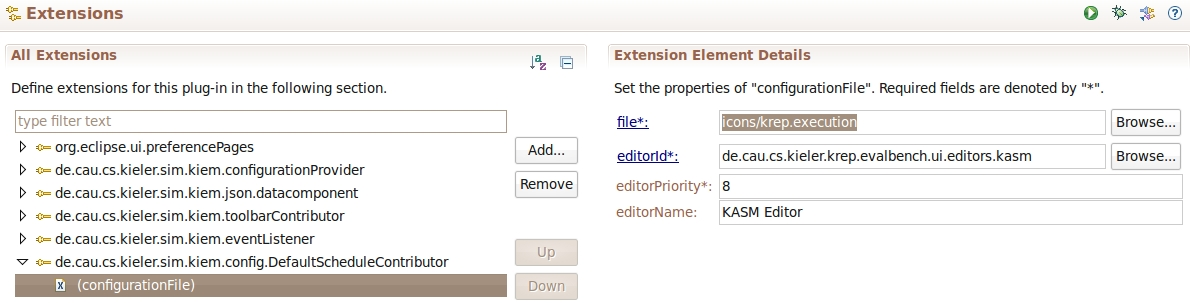
\includegraphics[scale=0.33]{DefaultSchedule.jpg}
  \caption[The Default Schedule extension point]%
  {The Default Schedule extension point with example\protect}
  \label{fig:DefaultSchedule}
\end{figure}

As soon as the Schedule Manager loads the schedules from the Eclipse preference store it also triggers
a load from the components registered on this extension point. The new schedule will be constructed with
the location provided through the corresponding field in the extension point. When a programmer decides
to provide the user with a default schedule he also has to provide an editor for that schedule
The extension point takes location of the execution file which will be assigned to an 

TODO:
\begin{itemize}
 \item all schedule data
 \item track recently used schedule Ids
 \item ask KIEMPlugin to load a saved schedule, deal with error
 \item add/remove schedules, update schedule priorities
 \item handle user load/save events
\end{itemize}


\subsection{Editor Manager}
\label{section:EditorManager}
\index{Editor Manager}
As described in Section \ref{section:EditorDefinition} the editor names and editor ids have to be saved
since they might not be available in the current runtime environment. The Editor Manager is responsible
for managing the list of all known editors. It also contains facilities around the default editor.

\begin{description}
 \item \textbf{EditorDefinition addEditor(EditorDefinition editor} : Adds a new editor to list of 
editors and return the added editor. If an editor with that editor id already exists in the list it is
not added to prevent duplicates. In this case the already existing editor is returned instead. Since
some methods may want to work on the editor that was just added they can work on the returned reference
instead of having to perform a find to get the correct object.
 \item \textbf{EditorDefinition findEditorById(String id)} : This method searches through the list
of available editors to retrieve the editor with the given id. Since editors ids are assumed to be
unique the first match is returned. This method is for example used to build the list of schedules that
work with the currently active editor.
 \item \textbf{void removeEditor(EditorDefinition editor)} : At some point the user may decide that
one of the editors is no longer used. In this case the editor is simply removed from the list of
available editors. However if the removed editor is the default editor (see Section \ref{section:DefaultEditor})
the method also has to choose a new default editor. The editor of choice for simplicity is the first
editor in the list. If the last editor is removed a hard-coded default editor is restored.
\end{description}

When the user is finished changing the editors the manager can use the facilities in the super class to
write the list of known editors to the Eclipse preference store.


\subsubsection{Default Editor}
\label{section:DefaultEditor}
\index{Default Editor}
The \ac{KIEMConfig} contains a facility for showing the list of schedules that match the currently active
editor. However there may be situations no editor is opened. Since the user should be able to keep working
with his schedules in this situation there is the need to define a default editor. This editor will be assumed open 
when in fact no editor is active.

Although the actual storing of the default editor happens inside the Configuration Manager the Editor Manager
still supplies facilities to get and set the default editor. This arrangement is more intuitive than having
the methods inside the Configuration Manager.


\subsection{Contribution Manager}
\label{section:ContributionManager}
\index{Contribution Manager}
The Contribution Manager is responsible for maintaining the view elements (see Section \ref{section:ConfigurationSelector}) 
that are not part of any of the preference pages. To accomplish this the manager has two tasks:
\begin{enumerate}
 \item The manager must create the view elements and store them. As described in Section 
\ref{section:ToolbarContributionProvider} the Execution Manager will ask the \ac{KIEMConfig}
for the list of items it wants to contribute to the tool bar. The manager then has to 
create the list with the saved view elements and forward it through the extension point.
 \item As the user might want to hide the new elements the Contribution Manager also has to 
keep track of the visibility of the elements. Showing and hiding the components is realized
in the following way:
\begin{itemize}
 \item When the Execution Manager requests the list of control contributions the Contribution Manager
checks whether or not the given view element should be visible. If it should not be shown on the tool bar
it is not added to the list and thus never reaches the tool bar.
 \item When the user changes the visibility of a given view element the manager first updates its own
representation of that information and triggers a save into the Eclipse preference store through the use
of the facilities in the super class. After that the manager triggers a refresh in the Execution Manager
view which causes the method in the extension point to be called which then receives the changed list.
\end{itemize}
\end{enumerate}

MAYBE TODO:
Advanced user mode


\subsection{Property Usage Manager}
\label{section:Property Usage Manager}
\index{Property Usage Manager}
As described in Section \ref{section:ConfTaskDefaultConfig} the user might not want to use
the properties saved in the currently loaded execution file but rather the default values
entered through the preference page. The Property Usage Manager is responsible enabling
the Configuration Manager to realize this feature.

To accomplish this task the manager contains a list of property keys for those values
that should be taken from the default configuration. The list can be changed by any other
class when the user changes the preferences on which properties should be in it. The list
is also stored and loaded through the use of the facilities in the Abstract Manager.


\subsection{Implementing Classes}
\begin{itemize}
 \item tool bar provider: link to contribution manager, forward array of contributions
 \item configuration provider: link to configuration manager, forward requests
 \item event listener: handles events received by the configData component 
    listen to load/save events, can be disabled when KIEMConf is about to trigger load/save
\end{itemize}

\section{Preference Pages - the View}
\begin{itemize}
 \item place to easily configure settings, all KIELER preferences in one place
 \item integrated into eclipse look and feel
\end{itemize}

\subsection{Configuration page}
\begin{itemize}
 \item changing default configuration for internal properties
 \item check boxes for changing visibility of the combos
\end{itemize}

\subsubsection{User defined properties page}
\begin{itemize}
 \item adding/removing properties
 \item modified from msp, table view with providers
\end{itemize}

\subsubsection{Property usage dialog}
This dialog shown in figure \ref{fig:PropertyUsageDialog} is used for selecting which properties should always be taken
from the default configuration rather than the configuration component contained
in every .execution file.
The dialog used for this is a ListSelectionDialog which just receives the list of
all keys as input and the list of PropertyKeys from the PropertyUsageManager as default selection.
After the user is finished with selecting attributes and hit the 'Ok' Button the dialog
passes the new list of selected items back to the PropertyUsageManager.
\begin{figure}[PropertyUsageDialog]
  \centering
  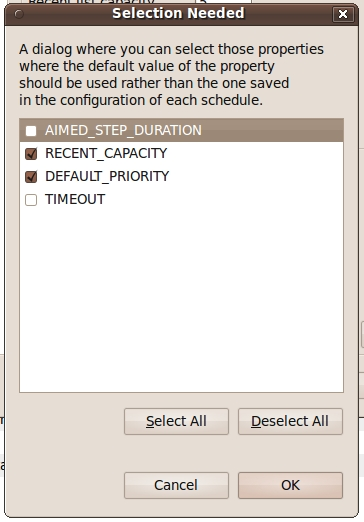
\includegraphics[scale=.5]{PropertyUsageDialog.jpg}
  \caption[Property Usage Dialog]%
  {The Property Usage Dialog\protect}
  \label{fig:PropertyUsageDialog}
\end{figure}

\subsection{Scheduling page}
This preference page is used to manage the schedules and the editors that they belong to.
This page is basically a modified version of the LayoutPrioritiesPage by msp.

\begin{itemize}
 \item table with schedules / editors and their priorities
 \item modified from msp , editors = diagram types, schedules = layouters
 \item modify priorities
 \item add/remove editors, remove schedules, selecting default editor
\end{itemize}

\subsubsection{Adding and removing editors, Selecting a default editor}
On the scheduling preference page there are routines for adding and removing
editors as well as selecting a default editor.
All of these actions use the same basic method for displaying an ElementListSelectionDialog \ref{fig:EditorSelectionDialog}
that takes a list of editor ids and returns the one selected by the user.
\begin{itemize}
 \item The editor adding dialog gets a list of all editors currently registered on the
 active workbench. The user can select a single editor which is then added to the table.
 \item The editor removal dialog gets a list of all editors currently available for 
 assignment of support properties. The editor selected by the user is removed from the table.
 It is also removed from all schedules. This is done to prevent the schedule objects from growing
 to monstrous size over time when editors are getting added and removed.
 \item The default editor selection dialog gets the same list as the removal dialog. The selected
 editor is then set as default editor. The default editor is used when there is no currently active editor on the workbench.
  It is used:
  \begin{enumerate}
   \item to determine which editors to show in the Matching combo box.
   \item when a new schedule is created as an editor id.
  \end{enumerate}
\end{itemize}
\begin{figure}[EditorSelectionDialog]
  \centering
  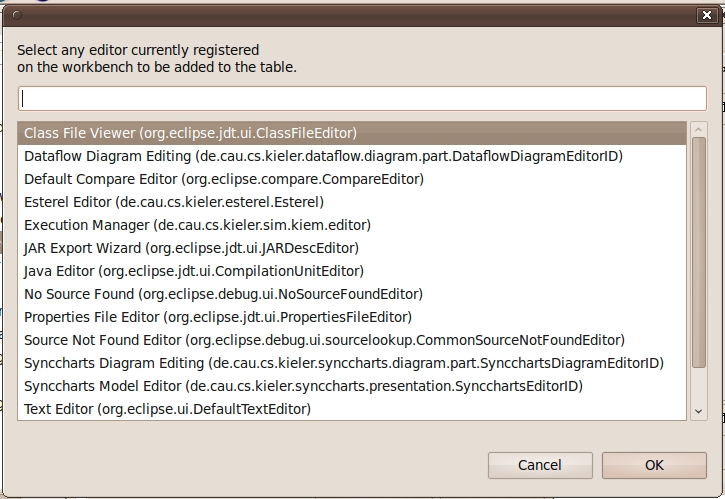
\includegraphics[width=1\textwidth]{EditorSelectionDialog.jpg}
  \caption[Editor Selection Dialog]%
  {The Editor Selection Dialog\protect}
  \label{fig:EditorSelectionDialog}
\end{figure}

\subsection{Configuration Selector}
\label{section:ConfigurationSelector}
\index{Configuration Selector}

